\chapter{Worksheets}
\label{ch:worksheets}

A workbook holds up to sixteen worksheets. Each has its own name, its own
cells, its own column widths and its own used range, and formulas on any of
them can read cells on any other.

All sixteen are saved in one \fname{.X16S} file. There is no way to save one
worksheet on its own, or to copy cells from one workbook into another.

\section{The tabs}
\index{worksheet!tabs}

Line 57 of the screen carries the tabs, ten characters each, the current one in
yellow.

\begin{ccfigure}
\ccscreenscale{1.5}
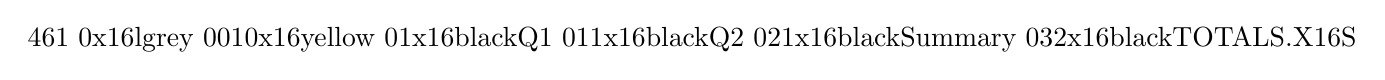
\begin{tikzpicture}
\node[inner sep=0pt,anchor=north west] (tb) at (0,0) {%
\ccscreenbegin{46}{1}
  \ccfillrow{0}{x16lgrey}
  \ccfill{0}{0}{10}{x16yellow}
  \cctext{0}{1}{x16black}{Q1}
  \cctext{0}{11}{x16black}{Q2}
  \cctext{0}{21}{x16black}{Summary}
  \cctext{0}{32}{x16black}{TOTALS.X16S}
\ccscreenend
};
\end{tikzpicture}
\caption{Three worksheets, with the workbook name after them}
\label{fig:tabs}
\end{ccfigure}

A name may be thirty-one characters long, but a tab is ten characters wide and
shows only the first nine. Long names are worth avoiding for that reason alone.

After the last tab, if the line has room left, \ccprod{} prints the name of the
workbook file.

\section{Moving between worksheets}
\index{worksheet!switching}

\begin{cctable}{To}{Do}{2.2in}{2.62in}
Go to the next worksheet & \menupath{Sheet > Next} \\
Go to the previous one & \menupath{Sheet > Previous} \\
Go to a particular one & Click its tab \\
\end{cctable}

\menupath{Next} and \menupath{Previous} wrap round: \menupath{Next} on the last
worksheet goes to the first.

\begin{ccnote}
Switching worksheets always puts the cursor on \cellref{A1}. It does not
remember where you were. This applies to the menu commands and to clicking a
tab.
\end{ccnote}

There is no keyboard shortcut for either command.

\section{Adding a worksheet}
\index{worksheet!adding}

\menupath{Sheet > Add\ccdots} asks for a name and adds a worksheet at the end.

\begin{ccfigure}
\ccscreenscale{1.15}
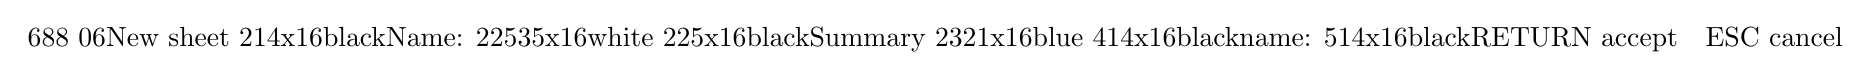
\begin{tikzpicture}
\node[inner sep=0pt,anchor=north west] (sa) at (0,0) {%
\ccscreenbegin{68}{8}
  \ccdlgbox{0}{6}{New~sheet}
  \cctext{2}{14}{x16black}{Name:}
  \ccfill{2}{25}{35}{x16white}
  \cctext{2}{25}{x16black}{Summary}
  \ccfill{2}{32}{1}{x16blue}
  \cctext{4}{14}{x16black}{name:}
  \cctext{5}{14}{x16black}{RETURN~accept~~~ESC~cancel}
\ccscreenend
};
\end{tikzpicture}
\caption{Adding a worksheet}
\label{fig:sheetadd}
\end{ccfigure}

The new worksheet is created but \emph{not} switched to. You stay where you
were; use \menupath{Sheet > Next} or click the new tab to go there.

An empty name cancels. Adding a seventeenth worksheet fails with
\msg{Resource limit reached}.

\section{Renaming a worksheet}
\index{worksheet!renaming}

\menupath{Sheet > Rename\ccdots} asks for a new name for the \emph{current}
worksheet, with the existing name already in the field so you can edit it.

Renaming a worksheet does not change any formula that refers to it, and a
formula naming a worksheet that no longer exists under that name is not
re-checked --- it keeps its last calculated value. If you rename a worksheet
that other worksheets read from, check them.

\section{Deleting a worksheet}
\index{worksheet!deleting}

\menupath{Sheet > Delete} removes the current worksheet and everything on it.

\begin{ccfigure}
\ccscreenscale{1.15}
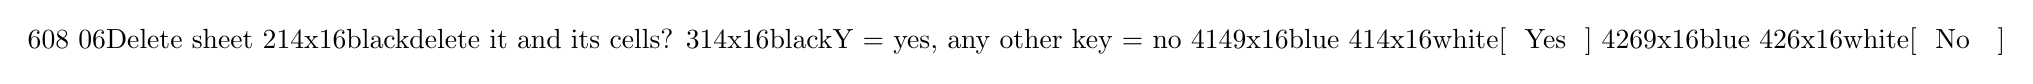
\begin{tikzpicture}
\node[inner sep=0pt,anchor=north west] (sd) at (0,0) {%
\ccscreenbegin{60}{8}
  \ccdlgbox{0}{6}{Delete~sheet}
  \cctext{2}{14}{x16black}{delete~it~and~its~cells?}
  \cctext{3}{14}{x16black}{Y~=~yes,~any~other~key~=~no}
  \ccfill{4}{14}{9}{x16blue}
  \cctext{4}{14}{x16white}{[~~Yes~~]}
  \ccfill{4}{26}{9}{x16blue}
  \cctext{4}{26}{x16white}{[~~No~~~]}
\ccscreenend
};
\end{tikzpicture}
\caption{Confirming a worksheet deletion}
\label{fig:sheetdel}
\end{ccfigure}

\begin{cccaution}
There is no undo for this. \key{F5} does not bring a deleted worksheet back;
nothing does. The confirmation box is the whole of the safety net.
\end{cccaution}

The last worksheet cannot be deleted --- a workbook must have at least one.

\section{Formulas across worksheets}
\index{formulas!cross-sheet}\index{worksheet!references between}

A cell reference may name a worksheet, with an exclamation mark between the
name and the reference.

\begin{ccexamples}[Cross-sheet references]{0.44\linewidth}
\exn{=Q1!B5}{}{cell B5 on the worksheet Q1}
\exn{=SUM(Q1!B2:B40)}{}{a range on another worksheet}
\exn{='My Data'!A1}{}{quotes are needed for a name with a space}
\end{ccexamples}

The name is matched without regard to case and must match the whole stored
name. Unquoted names may contain letters, digits, underscores and full stops;
anything else --- a space, or a leading digit --- needs single quotes.

\begin{ccnote}
The prefix applies to exactly one reference and no further. In
\fml{='My Data'!A1+A3}, \cellref{A1} comes from \emph{My Data} and
\cellref{A3} comes from the worksheet the formula is on. This trips people up;
write \fml{='My Data'!A1+'My Data'!A3} if that is what you meant.
\end{ccnote}

A formula naming a worksheet that does not exist is refused when you enter it,
in the same silent way as any other bad reference.

\subsection{Recalculation is workbook-wide}

Every recalculation sweeps every worksheet, not just the one you are looking
at. A chain of formulas that runs from \emph{Q1} through \emph{Q2} to
\emph{Summary} settles correctly however the cells are ordered and whichever
sheet you are on. Chapter~\ref{ch:recalc} explains how.
